\documentclass[tikz]{standalone}
\usetikzlibrary{automata,positioning}
\begin{document}

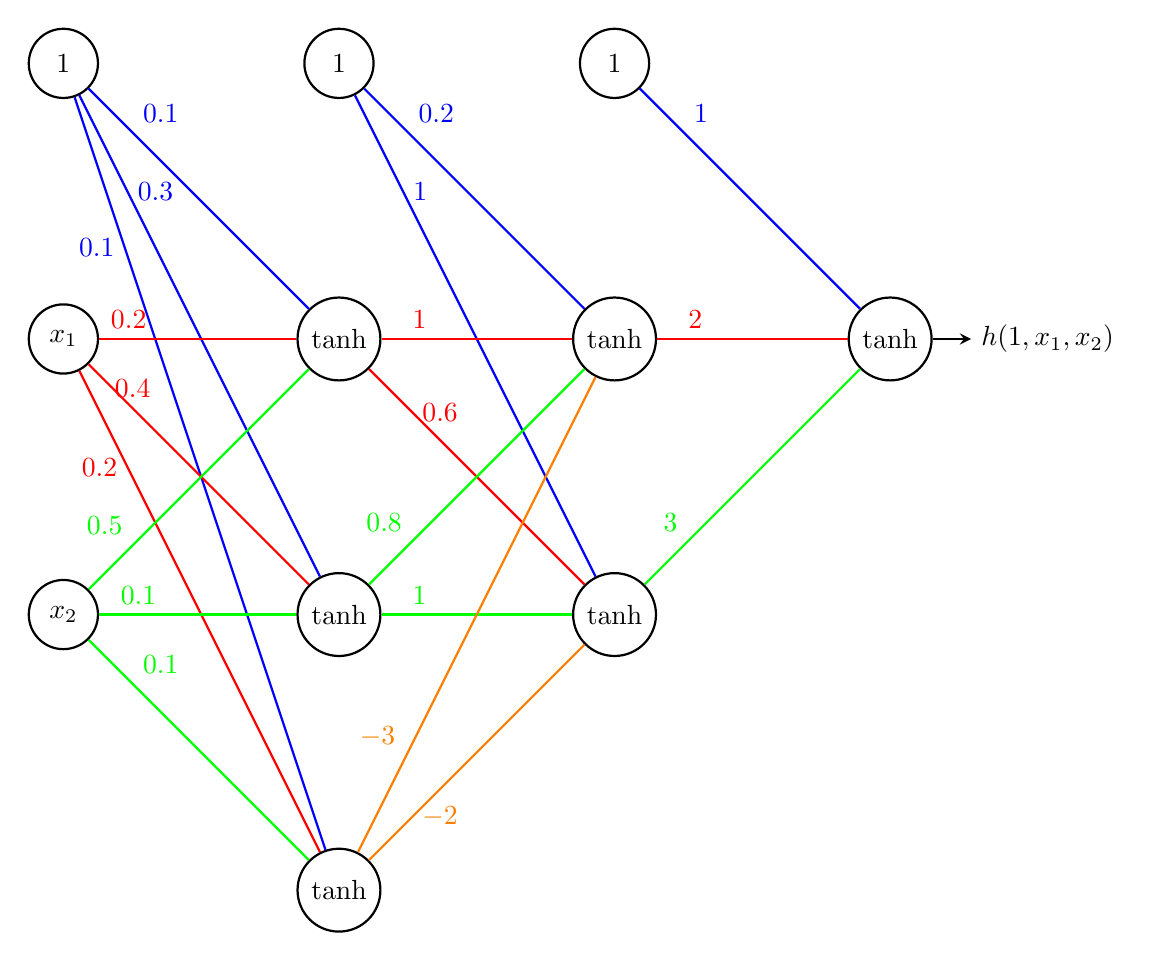
\begin{tikzpicture}[>=stealth,node distance=3.5cm,on grid,auto, thick, initial text=] 
  \node[state] (b0) {$1$};
  \node[state] (x1) [below=of b0] {$x_1$};
  \node[state] (x2) [below=of x1] {$x_2$};
  
  \node[state] (b1) [right=of b0] {$1$};
  \node[state] (n1) [below=of b1] {tanh};
  \node[state] (n2) [below=of n1] {tanh};
  \node[state] (n3) [below=of n2] {tanh};

  \node[state] (b2) [right=of b1] {$1$};
  \node[state] (n4) [below=of b2] {tanh};
  \node[state] (n5) [below=of n4] {tanh};

  %\node[state] (b3) [right=of b2] {$1$};
  \node[state] (o) [right=of n4] {tanh};

  \node (h) [right= 2cm of o] {$h(1,x_1,x_2)$};

  \path[-]
  (b0) edge [blue] node [pos=0.2] {$0.1$} (n1)
  (b0) edge [blue] node [right, pos=0.2] {$0.3$} (n2)
  (b0) edge [blue] node [left, pos=0.2] {$0.1$} (n3)
  
  (x1) edge [red] node [pos=0.15] {$0.2$} (n1)
  (x1) edge [red] node [above, pos=0.2] {$0.4$} (n2)
  (x1) edge [red] node [left, pos=0.2] {$0.2$} (n3)

  (x2) edge [green] node [pos=0.2] {$0.5$} (n1)
  (x2) edge [green] node [pos=0.2] {$0.1$} (n2)
  (x2) edge [green] node [pos=0.2] {$0.1$} (n3)

  
  (b1) edge [blue] node [pos=0.2] {$0.2$} (n4)
  (b1) edge [blue] node [right, pos=0.2] {$1$} (n5)

  (n1) edge [red] node [pos=0.2] {$1$} (n4)
  (n1) edge [red] node [right, pos=0.2] {$0.6$} (n5)

  (n2) edge [green] node [pos=0.2] {$0.8$} (n4)
  (n2) edge [green] node [pos=0.2] {$1$} (n5)

  (n3) edge [orange] node [pos=0.2] {$-3$} (n4)
  (n3) edge [orange] node [right, pos=0.2] {$-2$} (n5)

  (b2) edge [blue] node [pos=0.2] {$1$} (o)
  (n4) edge [red] node [pos=0.2] {$2$} (o)
  (n5) edge [green] node [pos=0.2] {$3$} (o)
  ;

  \path[->] (o) edge node {} (h);
\end{tikzpicture}
\end{document}